\documentclass[a4paper,12pt,answers,noaddpoints]{exam}

\usepackage[utf8]{inputenc}
\usepackage{listings}             % Include the listings-package
\usepackage[T2A]{fontenc}
\usepackage[english,russian]{babel}
\usepackage[warn]{mathtext}
\usepackage[]{authblk}
\usepackage[a4paper,margin=2cm]{geometry}
\usepackage[usenames]{color}
\usepackage{colortbl}
\usepackage{graphicx}
\usepackage{verbatim}
\usepackage{multirow}

% определение окружения для ответа
\renewcommand{\solutiontitle}{\noindent\textbf{Ответ:}\par\noindent}
\SolutionEmphasis{\itshape}
% нижний колонтитул
\cfoot[]{Лист \thepage\ из \numpages}
\headrule
% верхний колонтитул
\header{Lab 1}{\today}{Улыбина З.А.}

\usepackage{datetime}
\usepackage{graphicx}
\usepackage{amsmath, amssymb, amscd}
\usepackage{arydshln}
\usepackage{indentfirst}
\usepackage{appendix}
\usepackage{ifthen}
\usepackage{ifpdf}
\usepackage{url}
\ifpdf
  \usepackage[pdftex,unicode=true]{hyperref}
\else
  \usepackage[dvips,unicode=true]{hyperref}
\fi
\begin{document}
\title{Лабораторная работа №1 \\ Точечное оценивание моментов случайной величины}

% автор и его контакты
\author{
	\textit{Улыбина З.А., вар. 15}
	   }

\affil{СПбГУАП, Институт вычислительных систем и программирования}

\date{\today}

\maketitle
% номер 
\pagebreak
\section{Цель работы}
Ознакомление со способами моделирования случайных чисел с заданным законом распределения в современных математических пакетах, получение навыков нахождения выборочных моментов случайной величины и получение навыков наглядного представления результатов статистической обработки данных.
\section{Биномиальное распределение}
\begin{equation}
    F_Y(y) \equiv \mathbb{P}(Y \leqslant y) = \sum\limits_{k=0}^{\lfloor y \rfloor} \binom{n}{k}\, p^k q^{n-k},\; y \in\mathbb{R}
\end{equation}
\begin{figure}[h]
\centering
\begin{minipage}[h]{0.9\linewidth}
\caption{Плотность распределения}
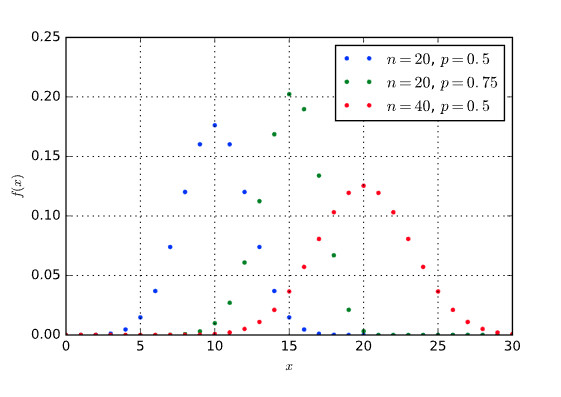
\includegraphics[width=0.7\linewidth]{1.jpg}
\end{minipage}
\vfill
\begin{minipage}[h]{0.9\linewidth}
\caption{Функция распределения}
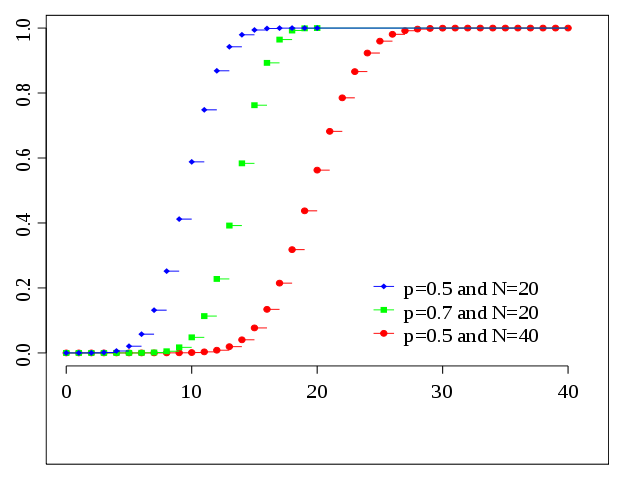
\includegraphics[width=0.7\linewidth]{2.png}
\end{minipage}
\end{figure}

\pagebreak

\section{Листинг кода}
\begin{verbatim}
#!/usr/bin/env python
# -*- coding: utf-8 -*-

# --- импорт необходимых модулей
import math
import numpy as np
import random
import matplotlib.pyplot as plt

# --- Биномиальное распределение
N = 20                                      # --- Заданный параметр распределения
P = 0.2                                     # --- Заданный параметр распределения
M = N * P                                   # --- Теоретическое матожидание
D = N * P * (1 - P)                         # --- Теоретическая дисперсия


COUNT_ELEMENT = 1000                        # --- Количество элементов в выборке
COUNT_ROUNDS = 100                          # --- Количество раундов получения выборок

# --- массивы для хранения данных для построения графиков:
means_all = []                              # --- математические ожидания
disp_all = []                               # --- дисперсии
means_error_all = []                        # --- кв. ошибок матожданий
disps_error_all = []                        # --- кв. ошибок дисперсий

# --- генерация данных
for i in range(COUNT_ROUNDS):               # --- в этом цикле получаем выборки
    tmp_sum = 0                             # --- здесь хранится текущая сумма

    # --- создаем выборку из COUNT_ELEMENT элементов:
    random_array = np.array([np.random.binomial(N, P) for i in range(COUNT_ELEMENT)])

    # --- врЕменные массивы (для соответствующих параметров):
    tmp_means = []
    tmp_error_means = []
    tmp_disps = []
    tmp_error_disps = []

    for i in range(COUNT_ELEMENT):          # --- в этом цикле считаем матожидания и дисперсии
        tmp_sum += random_array[i]          # --- обновляем сумму
        current_mean = tmp_sum / (i + 1.0)    # --- вычисляем текущее среднее
        tmp_means.append(current_mean)      # --- добавляем в соответствующий массив

        # --- вычисляем квадрат ошибки среднего и записываем
        tmp_error_means.append((current_mean - M) ** 2)

        # --- вычисляем второй центральный момент
        current_disp = sum((random_array[:i] - current_mean) ** 2) / (i + 1)
        tmp_disps.append(current_disp)      # --- записываем его

        # --- вычисляем квадрат ошибки дисперсии и записываем
        tmp_error_disps.append((current_disp - D) ** 2)

    # --- добавляем временные массивы в глобальные:
    means_all.append(tmp_means)
    means_error_all.append(tmp_error_means)
    disp_all.append(tmp_disps)
    disps_error_all.append(tmp_error_disps)

    plt.plot(tmp_means) # --- здесь же рисуем средние

# --- рисуем линию для теоретического среднего:
plt.plot([M for i in range(COUNT_ELEMENT)], 'g--', linewidth=3.5)
# --- рисуем линии для границы 3 sigma:
plt.plot([M + 3.0 * math.sqrt(D / COUNT_ELEMENT) for i in range(COUNT_ELEMENT)], 'r--', linewidth=1.5)
plt.plot([M - 3.0 * math.sqrt(D / COUNT_ELEMENT) for i in range(COUNT_ELEMENT)], 'r--', linewidth=1.5)
plt.show() # --- cначала рисуем зависимость средних от N

# --- устанавливаем логарифмические масштабы по осям, основание 2
plt.xscale('log', basex=2)
plt.yscale('log', basey=2)
for i in range(COUNT_ROUNDS):
    plt.plot(means_error_all[i])
plt.show() # --- квадрат ошибки среднего от N

for i in range(COUNT_ROUNDS):
    plt.plot(disp_all[i])
# --- рисуем линию для теоретической дисперсии:
plt.plot([D for i in range(COUNT_ELEMENT)], 'g--', linewidth=3.5)
plt.show() # --- дисперсия от N

# --- устанавливаем логарифмические масштабы по осям, основание 2
plt.xscale('log', basex=2)
plt.yscale('log', basey=2)
for i in range(COUNT_ROUNDS):
    plt.plot(disps_error_all[i])
plt.show() # --- квадрат ошибки дисперсии от N

# --- осредненные графики:
mean = []  # --- для кв. ошибки матожидания
disp = []  # --- для кв. ошибки дисперсии
for i in range(COUNT_ELEMENT):
    tmp_sum_m = 0
    tmp_sum_d = 0
    for j in range(COUNT_ROUNDS):
        tmp_sum_m += means_error_all[j][i]
        tmp_sum_d += disps_error_all[j][i]
    tmp_sum_m /= COUNT_ROUNDS
    tmp_sum_d /= COUNT_ROUNDS

    mean.append(tmp_sum_m)
    disp.append(tmp_sum_d)

# --- устанавливаем логарифмические масштабы по осям, основание 2
plt.xscale('log', basex=2)
plt.yscale('log', basey=2)
plt.plot(mean)
plt.show() # --- квадрат ошибки среднего от N

# --- устанавливаем логарифмические масштабы по осям, основание 2
plt.xscale('log', basex=2)
plt.yscale('log', basey=2)
plt.plot(disp)
plt.show() # --- квадрат ошибки дисперсии от N
\end{verbatim}

\pagebreak
\section{Результаты моделирования}
\subsection{Математическое ожидание}
\begin{figure}[h!]
\centering
\begin{minipage}[h!]{1.1\linewidth}
\caption{Зависимость $\mu$ от $N$}
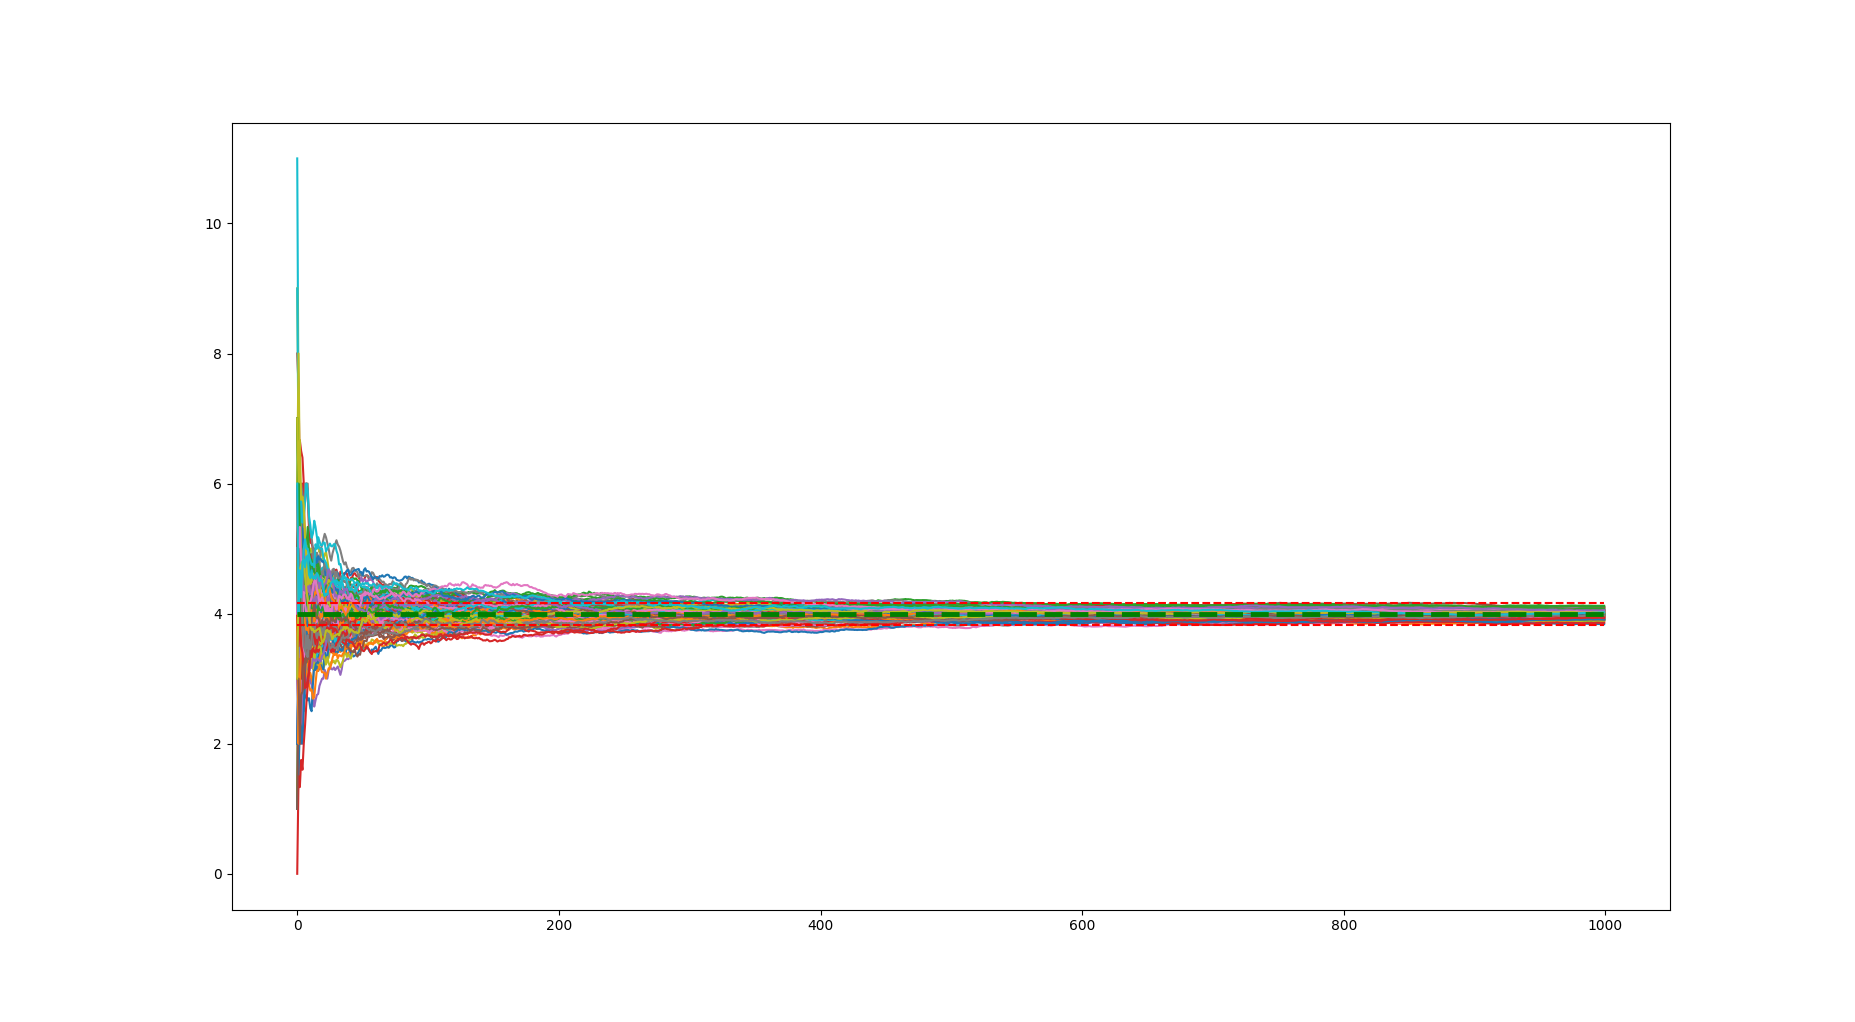
\includegraphics[width=1\linewidth]{../pngs/means_N.png}
\end{minipage}
\vfill
\begin{minipage}[h!]{1.1\linewidth}
    \caption{Квадрат ошибки $\mu(N)$}
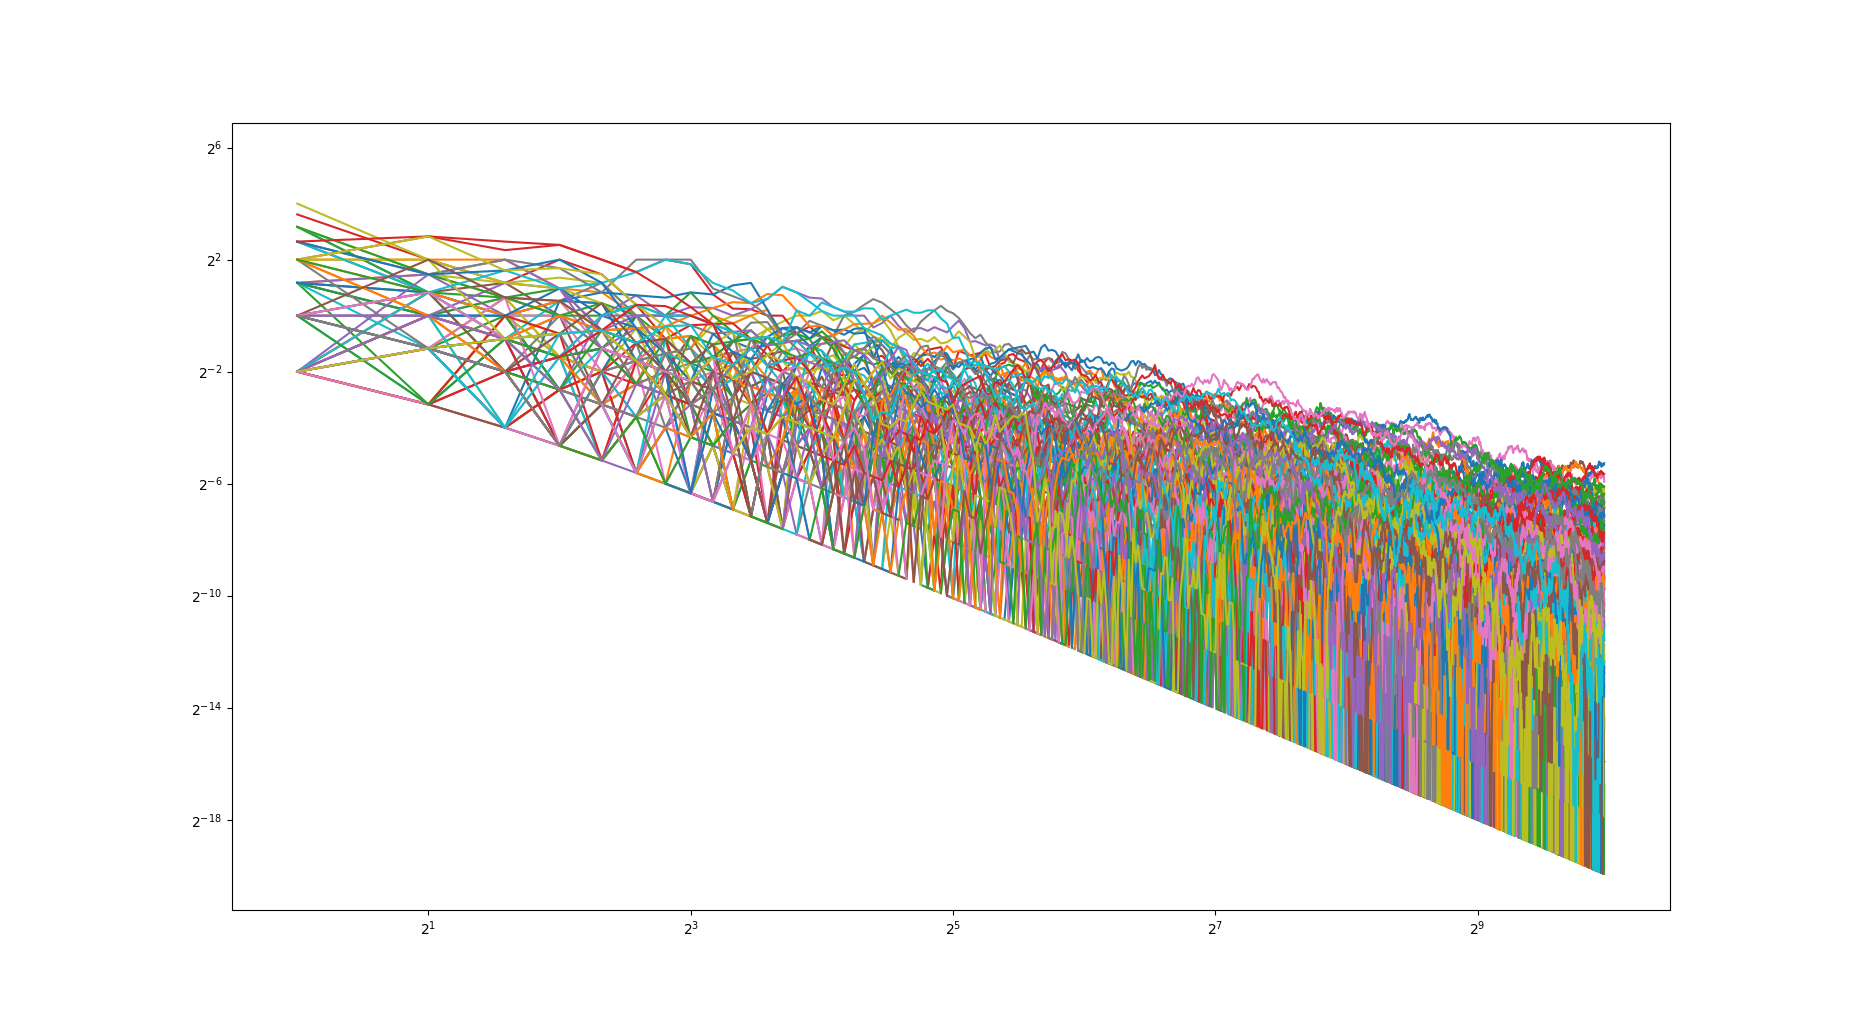
\includegraphics[width=1\linewidth]{../pngs/means_err.png}
\end{minipage}
\end{figure}
\pagebreak

\subsection{Дисперсия}
\begin{figure}[h!]
\centering
\begin{minipage}[h!]{1.1\linewidth}
\caption{Зависимость $D$ от $N$}
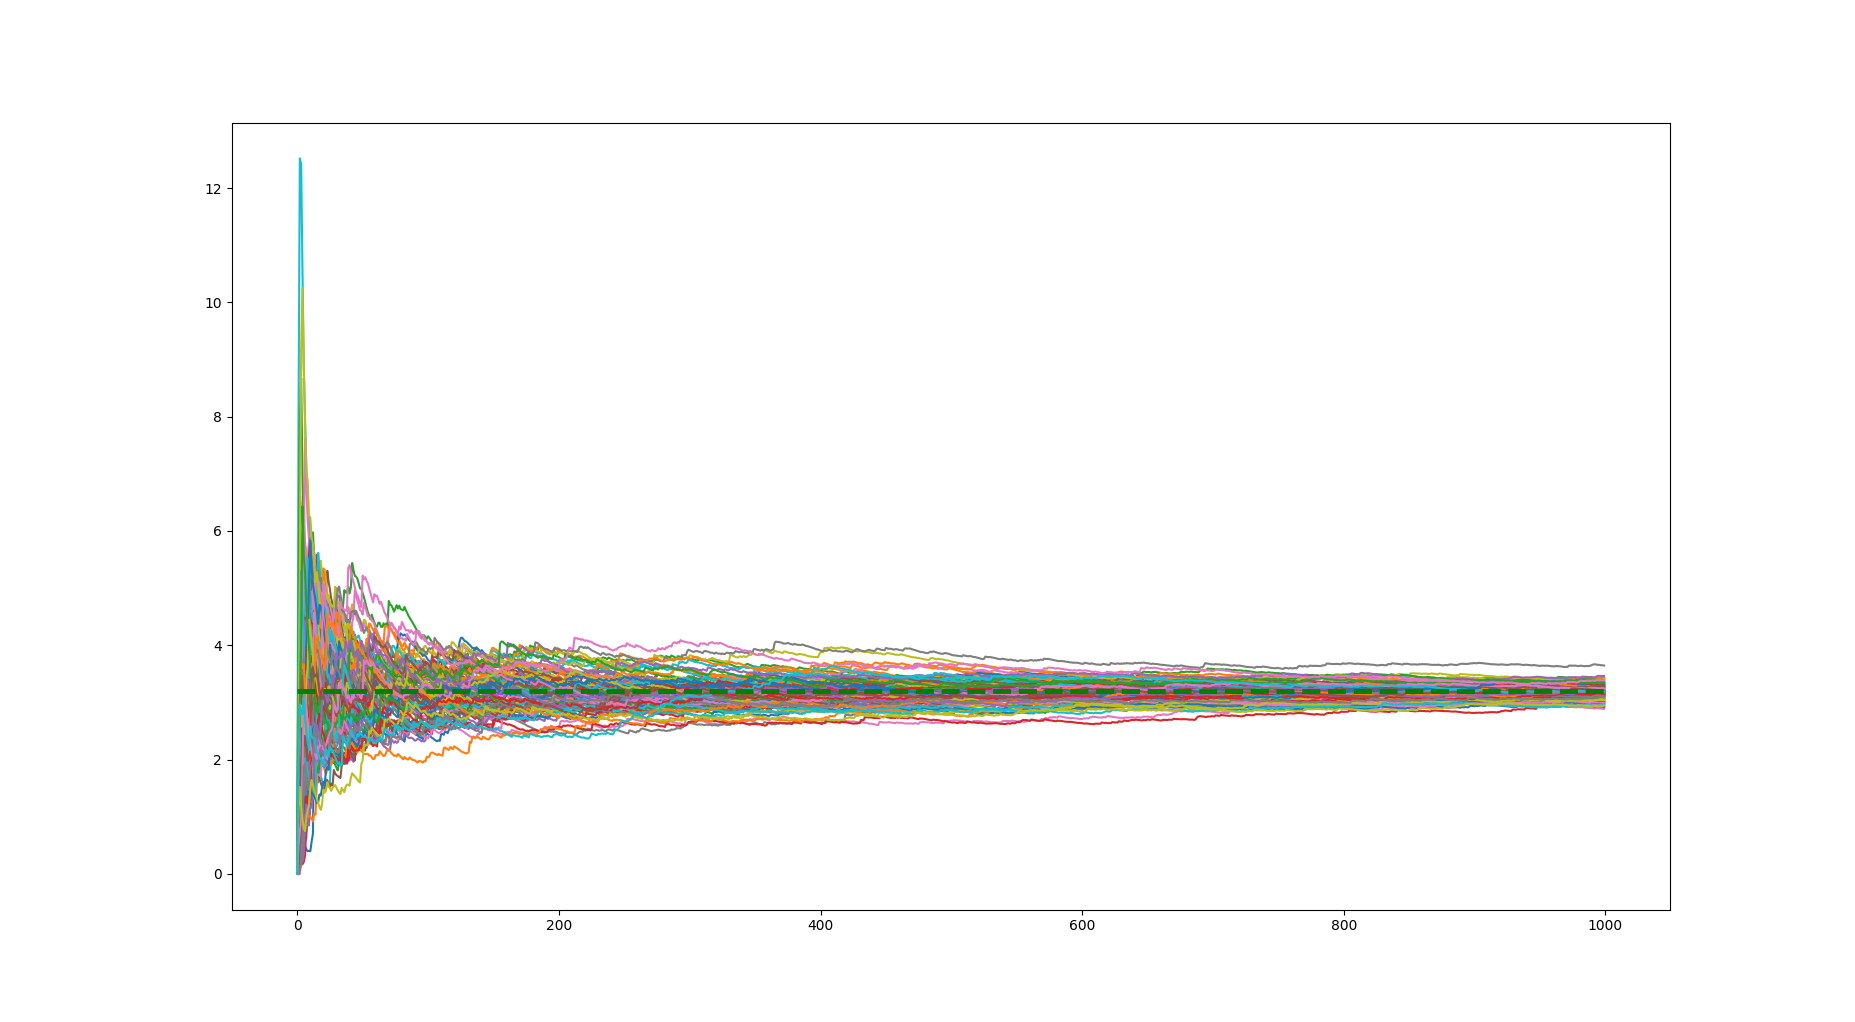
\includegraphics[width=1\linewidth]{../pngs/disp_N.png}
\end{minipage}
\vfill
\begin{minipage}[h!]{1.1\linewidth}
    \caption{Квадрат ошибки $D(N)$}
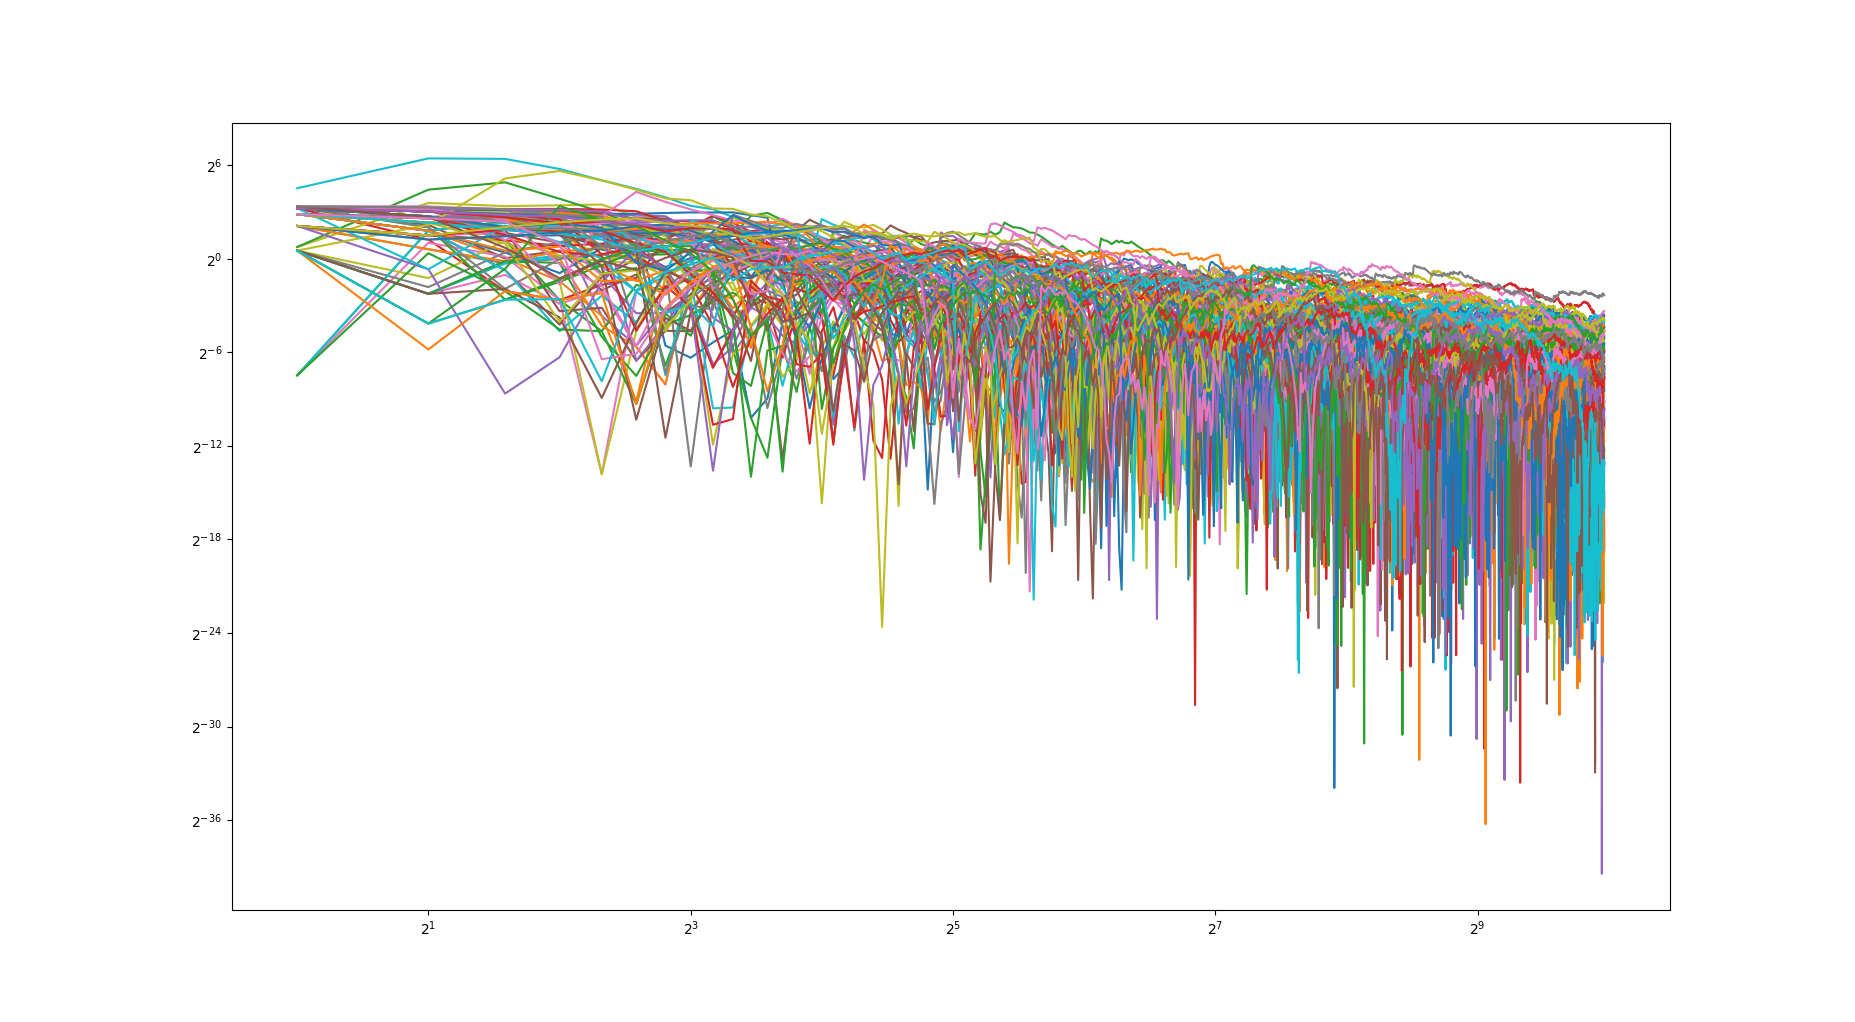
\includegraphics[width=1\linewidth]{../pngs/disps_err.png}
\end{minipage}
\end{figure}

\pagebreak
\subsection{Осредненные результаты}
\begin{figure}[h!]
\centering
\begin{minipage}[h!]{1.1\linewidth}
    \caption{Зависимость $e_{\mu}$ от $N$}
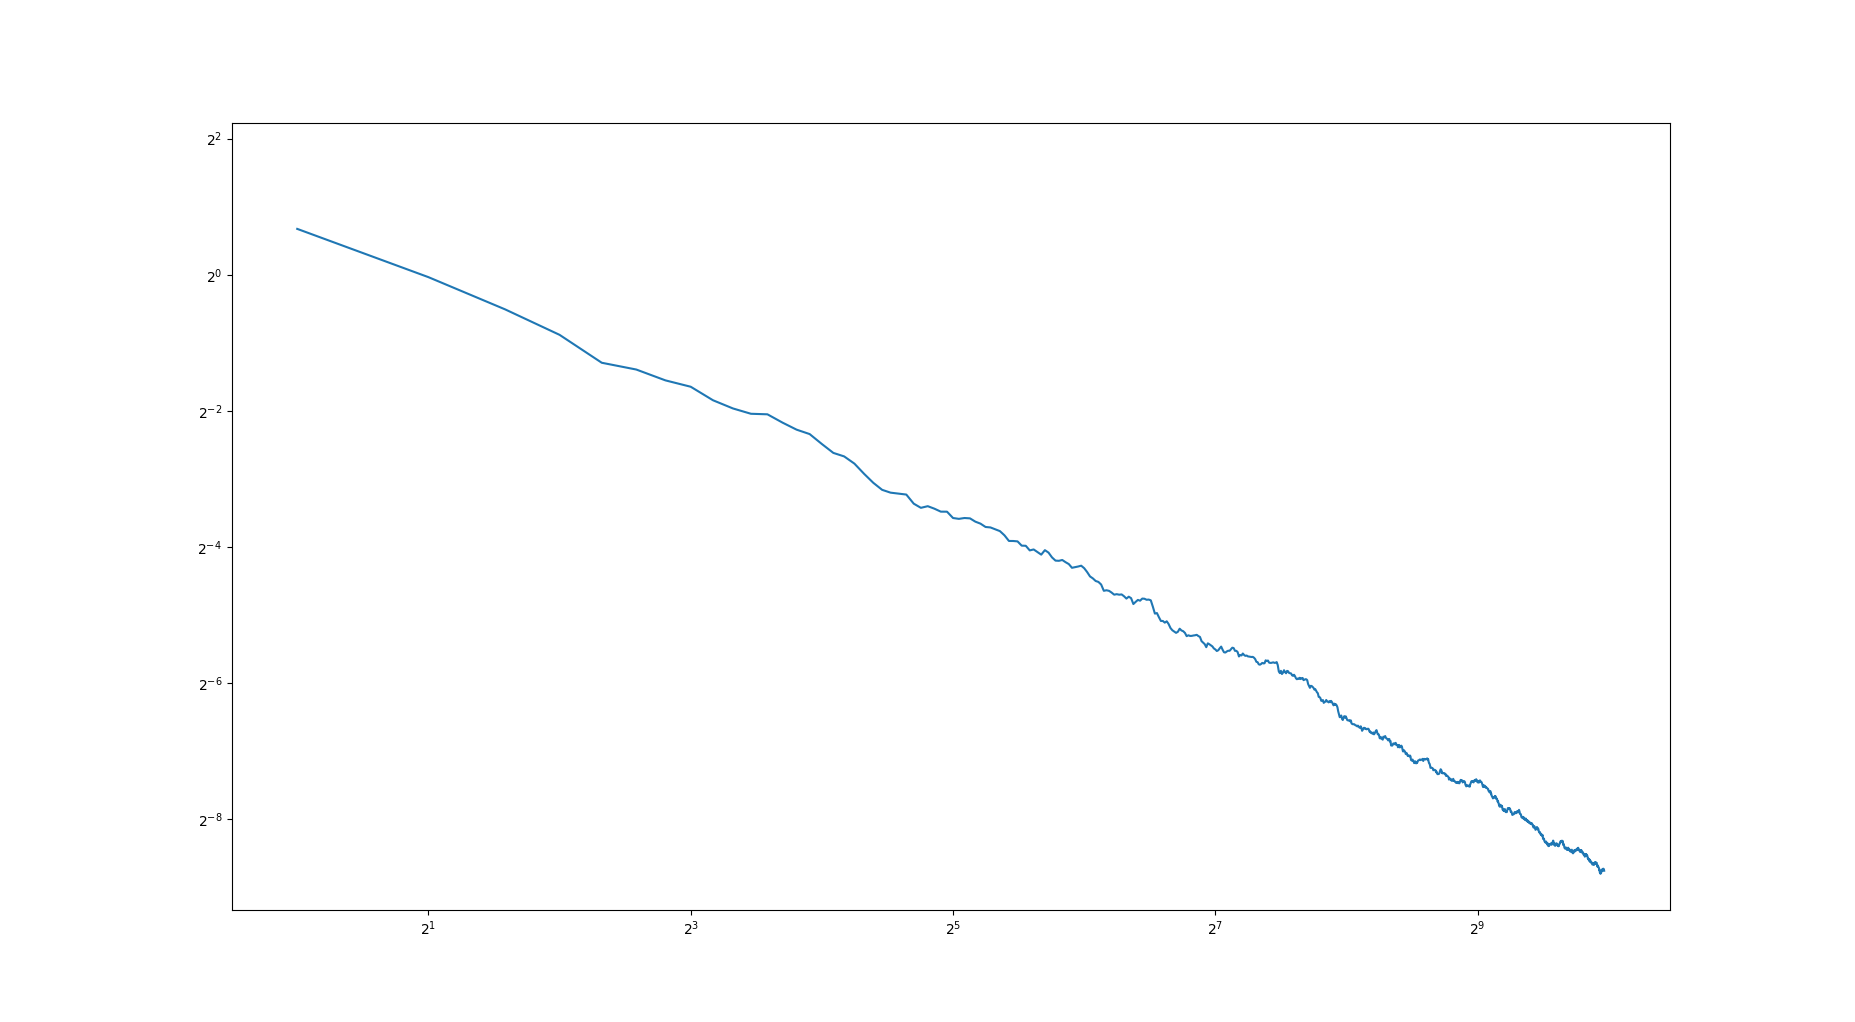
\includegraphics[width=1\linewidth]{../pngs/mean_errors_approx.png}
\end{minipage}
\vfill
\begin{minipage}[h!]{1.1\linewidth}
    \caption{Зависимость $e_{D}(N)$}
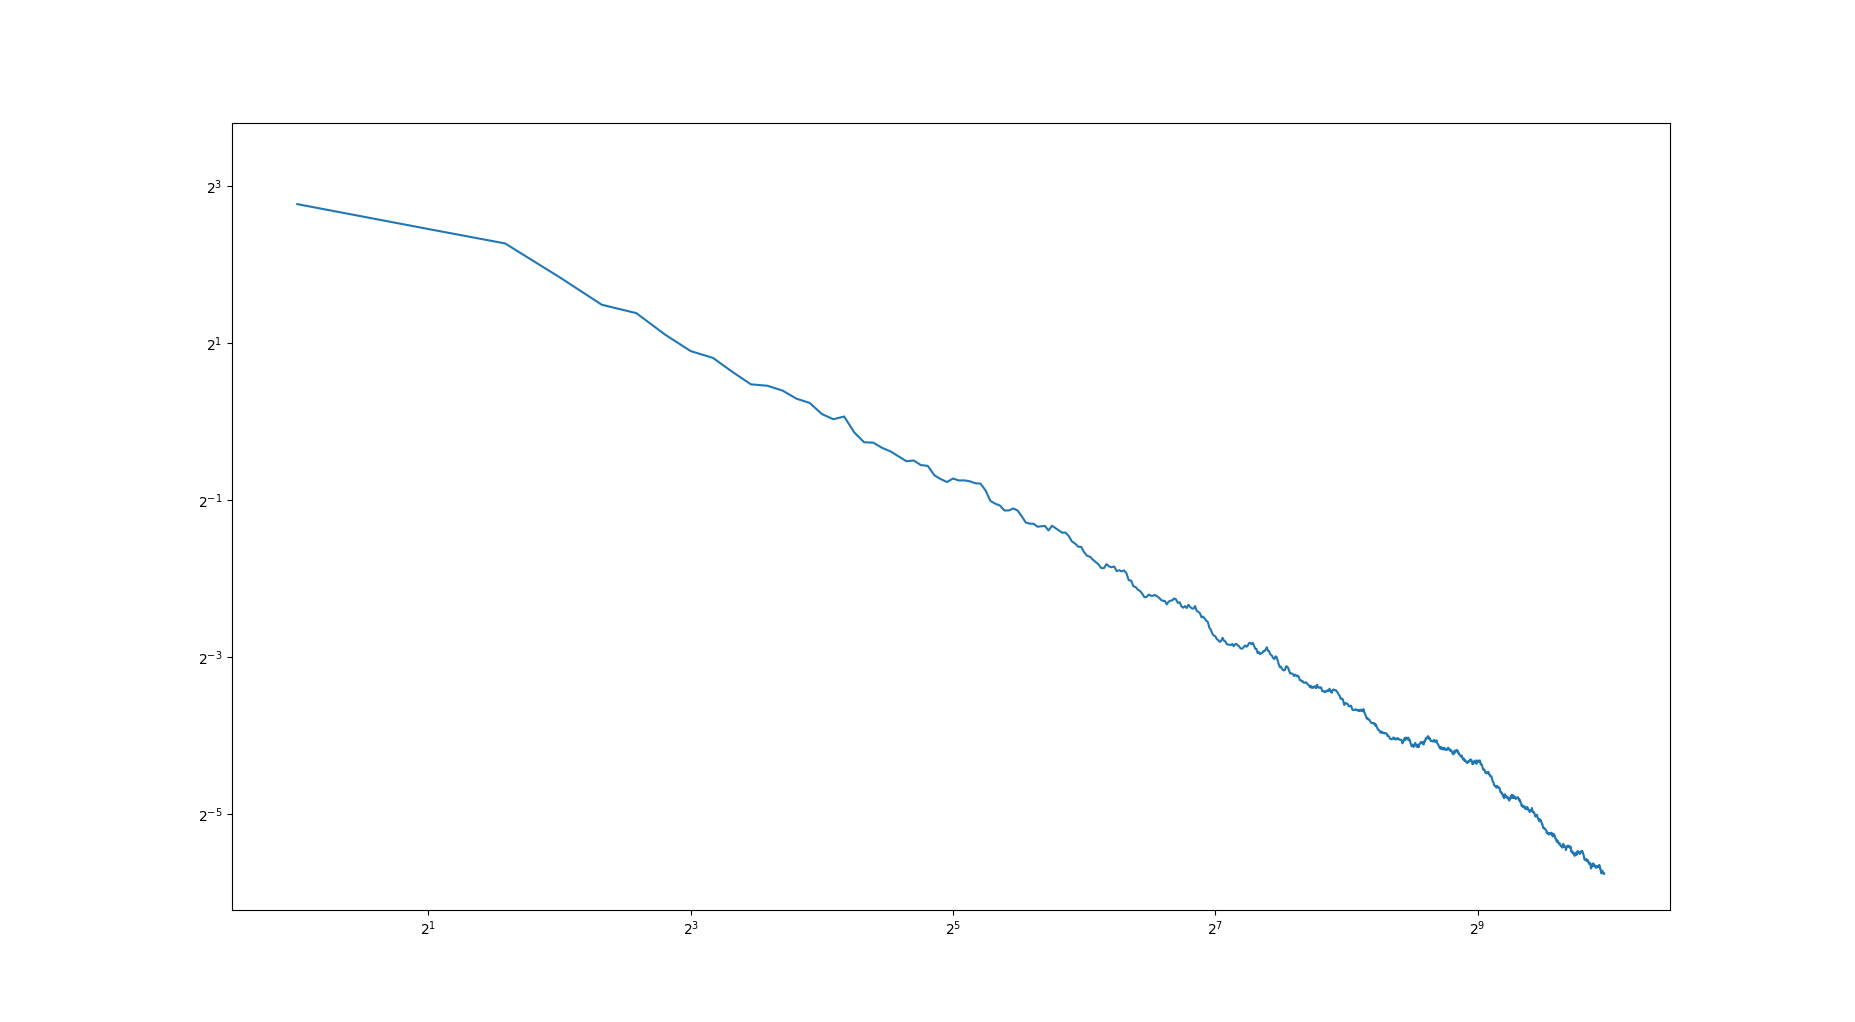
\includegraphics[width=1\linewidth]{../pngs/disp_errors_approx.png}
\end{minipage}
\end{figure}

\pagebreak
%%%%%%%%%%%%%%%%%%%%%%%%%%%%%%%%%%%%%%%%%%%%%%%%%%%%%%%%%%%%%%%%
\tableofcontents
\hfill
\end{document}
